\chapter{Application: prédiction d'entrée manquante}
\graphicspath{{05-Application/}}
\minitoc

Dans ce chapitre final, nous proposons une série d'expériences autour de tâches de prédiction de modalité par des structures de cartes CxSOM.
Nous nous placons dans un cadre d'application de mémoire associative.

L'une des motivations de la construction d'une architecture de cartes de Kohonen est de constuire des systèmes de cartes autonomes, notamment en robotique; c'est à dire, un système de carte capable d'effectuer de la prise de décision à partir des calculs effectués dans chaque carte, à savoir le calcul de BMU.
Dans un contexte de mémoire associative, cette prise de décision se rapporte à la prédiction d'une modalité à partir des autres modalités. Ces modalités étant dépendantes les unes des autres, nous attendons de cette prédiciton d'être en accord avec les autres entrées présentées à l'architecture.

Nous avons étudié comment des architectures CxSOM apprennent une représentation interne des relations entre modalités.
La capacité d'une architecture à prédire une modalité traduit l'existence de cette représentation interne.
Dans une architecture CxSOM, une carte ne recevant pas d'entrée externe possède une activité générée par ses entrées contextuelles.
Après apprentissage sur toutes les modalités, toutes les cartes ont des poids externes et contextuels dépliés.
Grâce aux entrées contextuelles, la présentation d'une entrée externe à seulement l'une des cartes permet à chaque carte de l'architecture d'avoir une activité et donc un BMU. Le poids externe de ce BMU peut alors être interprété comme une prédiction de la modalité correspondante.
Nous utiliserons cette propriété dans ce chapitre pour prédire la modalité relative à une carte. La qualité de cette prédiction témoignera de l'apprentissage d'une représentation interne cohérente par l'architecture de cartes. 
Ce chapitre propose une première application de CxSOM dans un cadre de prédiction d'entrée manquante. Nous étudierons comment cette prédiction est mise en oeuvre par l'architecture de cartes. Nous étudierons cette prédiction dans le cadre d'entrées géométriques, puis l'appliquerons à de la prise de décision pour la commande d'un drône.

\section{Prédiction d'entrées géométriques}

Avant d'effectuer des tâches de prédiction dans un cadre réel, nous réalisons des expériences sur les modèles d'entrées géométriques étudiés tout au long de la thèse
Nous étudierons ainsi la prédiction d'une modalité dans le cadre du cercle en 3D et de la sphère 3D. 
Nous prenons dans cette section des architectures de trois cartes connectées de façon rétroactive. 
Le but de 

\subsection{Algorithme de prédiction}

L'étape de prédiction est effectuée après apprentissage sur toutes les modalités.
Lors de la phase d'apprentissage, chaque carte de l'architecture possède une entrée externe. Après l'apprentissage, les poids sont figés.
Pour prédire une modalité $i$, les entrées externes de la carte ayant appris cette modalité ne lui sont plus présentées. Les autres cartes prennent quant à elles une entrée externe.
La carte ayant été "fermée" fait alors office de module de prédiction. Son activité est guidée par ses entrées contextuelles: l'activité globale est alors prise comme la moyenne des activités contextuelles. Le processus de relaxation est réalisé pour chaque entrée présentée à l'architetcture.
La carte correspondant à la modalité à prédire possède une couche de poids externes préalablement organisée lors de la phase d'apprentissage. Le poids externe du BMU, $\w\ext\m{i}(\bmu\m{i})$ est alors utilisé comme prédiction de la modalité manquante. 
Notons que la prédiction d'entrée par l'architecture CxSOM se passe d'utiliser un algorithme supplémentaire. Elle résulte de la dynamique du système de cartes. De cette façon, nous nous rapprochons de l'idée d'un système de carte autonome.

\begin{figure}
\centering
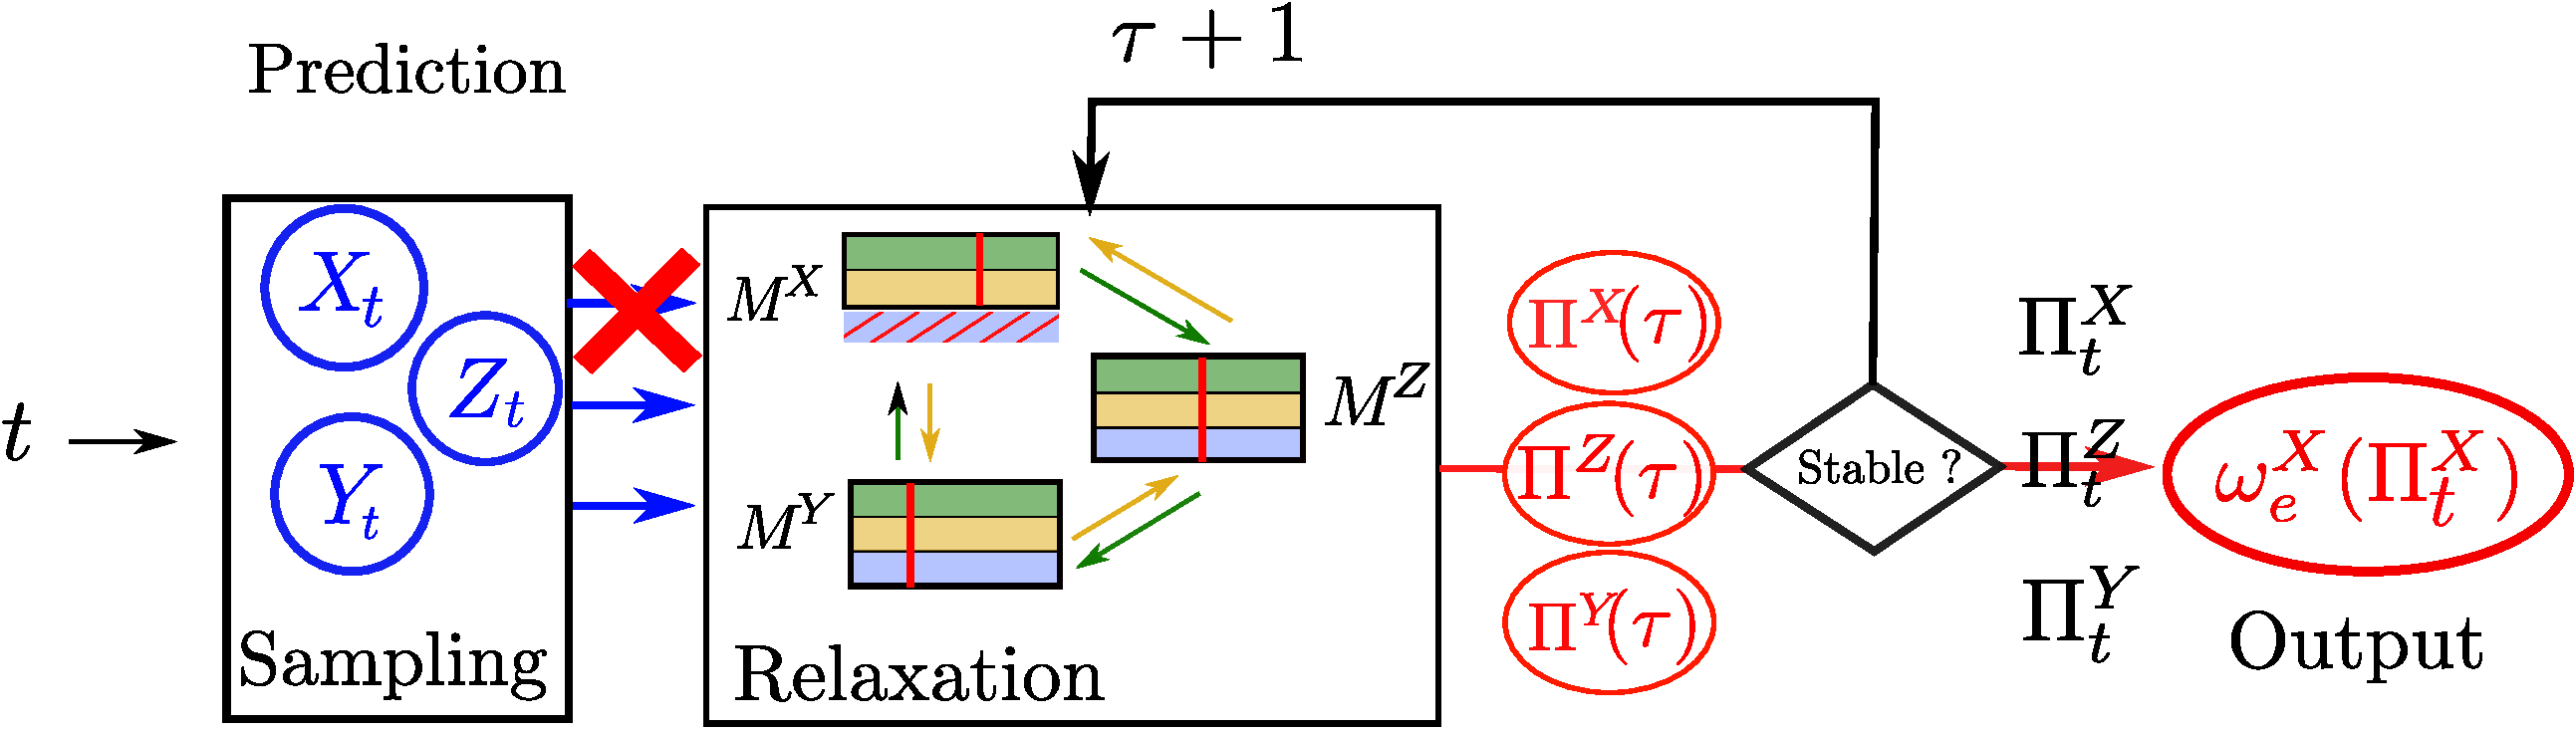
\includegraphics[width=\textwidth]{prediction_setup}
\caption{Description de l'algorithme de prédiction. Il s'agit du même algorithme que pour les tests, sans apprentissage, mais une modalité n'est pas présentée à l'architecture. Le poids externe du BMU de la carte correspondant à la modalité manquante est utilisé comme la prédiction de cette modalité.}
\label{fig:schema}
\end{figure}


\subsection{Résultats}
La figure \ref{fig:pred} représente la valeur de la prédicton $\w\ext\m{1}(\bmu\m{1})$ en fonction de la valeur théorique de cette entrée. 
\begin{figure}
\centering
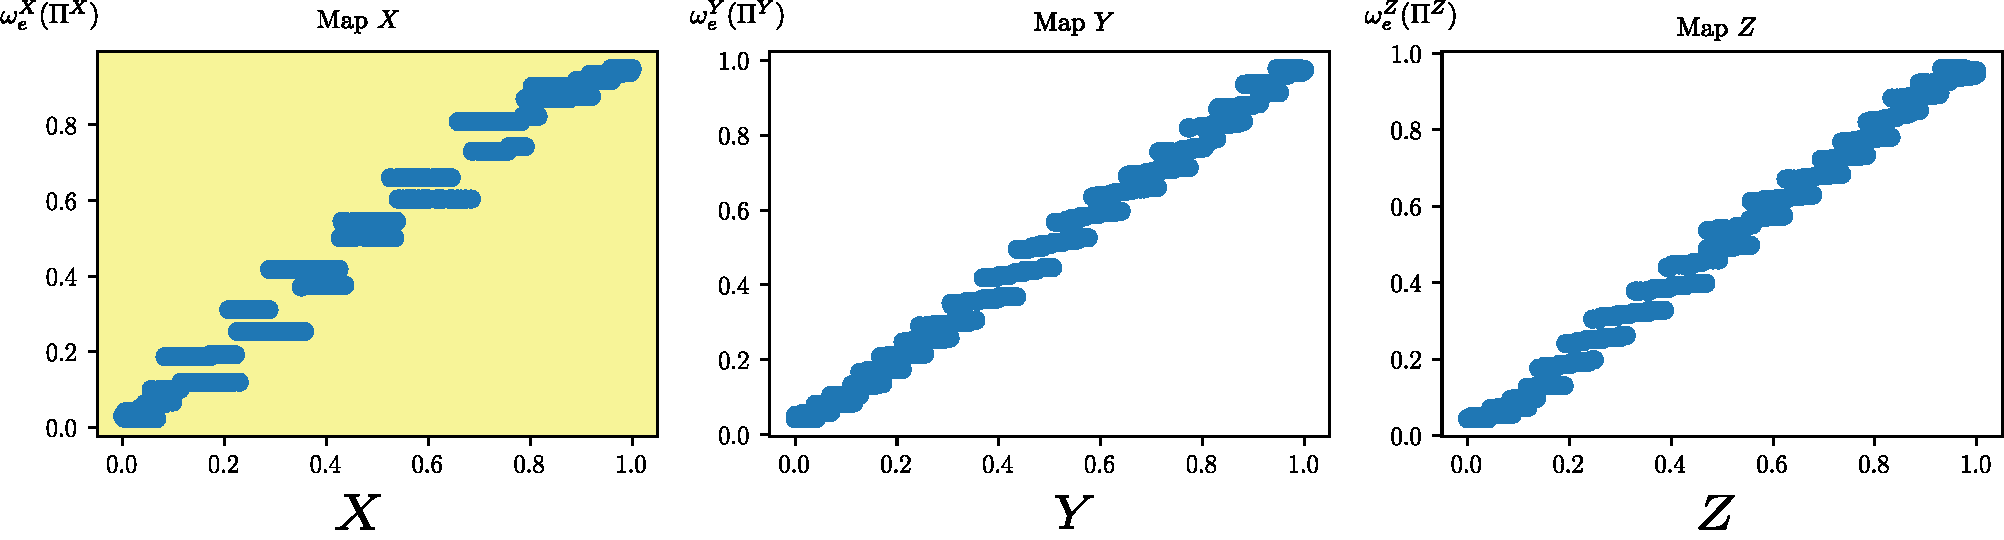
\includegraphics[width=\textwidth]{prediction_x2}
\caption{Prediction de x}
\label{fig:pred}
\end{figure}


\subsection{Discussion}
Les résultats sur des entrées géométriques montrent une bonne capacité de prédiction d'entrée.
La précision est limitée, mais on peut voir cette capacité de prédiction plus comme une preuve de mémoire associative que d'application pratique.
Ce qu'on cherche par la mémoire associative, c'est d'abord d'évoquer une modalité à partir d'autres. Ici, grâce à la connexion entre carte, on génère une zone de valeur limitée pour la modalité $X$: une région est activée, qui est reliée aux valeurs de $X$.
On va plutot parler d'évocation plutot que de prédiction. 

\section{Application à la commande de drône en vol}

Nous sortons du cadre des entrées simulées pour nous placer dans un cas de contrôle réel. Nous disposons d'un drône quadricoptère, commandé à distance. Ce drône possède une caméra frontale ainsi qu'un ensemble de capteurs internes. Chacun de ces capteurs peut être considéré comme une modalité d'un espace multimodal. A ces modalités s'ajoute la modalité correspondant à la commande envoyée au drône.
Le principe est d'apprendre, à l'aide d'une architecture de cartes, les relations existants entre les modalités des capteurs et de la commande afin d'ensuite prédire la commande à envoyer à partir des capteurs.
Afin que les relations entre la commande et les capteurs soient significatives, nous nous placons dans un cas d'application particulier: le drône vole dans un couloir étroit, en ligne droite. Le but du drône est alors de voler en avant dans le couloir, sans toucher les murs.
Le but de cette expérience est de démontrer la tâche de prédiction en situation réelle. Nous évaluerons ainsi la robustesse de l'algorithme à des données bruitées, et la capacité de CxSOM à réagir en temps réel malgré la relaxation.

\subsection{Méthode expérimentale}

Le drône utilisé pour l'expérience est un quadricoptère. Il possède une caméra frontale.
Le drône est contrôlé à distance par un ordinateur; la commande est réalisée en envoyant l'accélération angulaire du drône autour de ses trois axes de rotation.
Nous avons accès aux données des capteurs internes, notamment la vitesse linéaire courante selon chaque axe de déplacement.

le drône se déplace dans un couloir étroit.
Dans le cadre de l'expérience, nous extrayons deux éléments visuels spécifiques au couloir à partir de la caméra du drône: l'abscisse du point de fuite du couloir $x$. Nous calculons également la différence entre les angles du couloir, notée $\varphi$. Ces valeurs sont illustrées en figure~\ref{fig:drone}.
Le drône se déplace dans un couloir, à hauteur constante et vitesse constante.
La commande générant le déplacement en avant du drône (tangage) est maintenue constante. Les commandes permettant le déplacement en largeur sont alors $\omega$ et $\rho$. Dans le cadre de cette expérience, nous contrôlerons uniquement $\rho$.
Enfin, la vitesse linéaire en largeur du drône peut être récupérée à chaque instant; nous la notons $v$.
Nous avons ainsi quatres modalités lors du déplacement du drône: $x$, $\varphi$, $\rho$ et $v$.
Nous construisons une architecture CxSOM sur ces quatres modalités, composée de quatre cartes connectées chacune aux trois autres.
Une phase d'apprentissage est réalisée sur des déplacements du drône contrôlés humainement. Notons que lors de cette phase, nous avons utilisé un système de contrôle PID pour assister la commande humaine. Cette phase d'apprentissage est réalisée hors ligne pour que les données soient réparties aléatoirement.
Après apprentissage, nous effectuons une phase de prédiction. Lors de cette étape, la commande $\rho$ n'est plus présentée à la carte correspondante. Nous envoyons alors le poids externe du BMU de cette carte comme commande du drône. Cette étape est réalisée en ligne, sur des trajectoires réelles du drône.

La figure \ref{fig:drone_inp} présente la répartition des entrées présentées au drône. Nous avons tracé les dépendances entre chaque modalité. Nous remarquons sur la figure qu'une dépendance forte se dégage entre les entrées ?? et ??, ainsi que ?? et ??. Si les cartes apprennent correctement le modèle liant les entrées, la prédiction peut être réalisée.
Ces dépendances sont très bruitées. Cette expérience en conditions réelles nous permettra d'observer la résistance au bruit de la prédiction.

%TODO mettre disposition des entrées.

\subsection{Résultats}
La carte associée à $\rho$ possède donc une couche de poids externe et trois couches de poids contextuels. Ces poids sont représentés en figure \ref{fig:drone_w}. L'organisation des poids contextuels rappelle celle observé dans des conditions géométriques: les poids contextuels définissent des zones. Contrairement à l'expérience réalisée sur un cercle, la taille de ces zones dépend de la couche de poids contextuel définie. 

\begin{figure}
\begin{minipage}{0.5\textwidth}
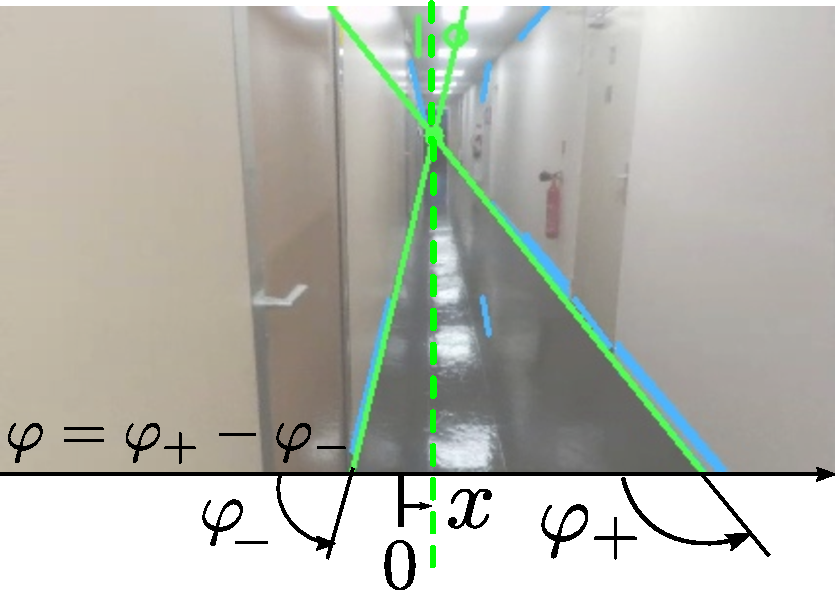
\includegraphics[width=\textwidth]{visudrone}
\end{minipage}
\begin{minipage}{0.5\textwidth}
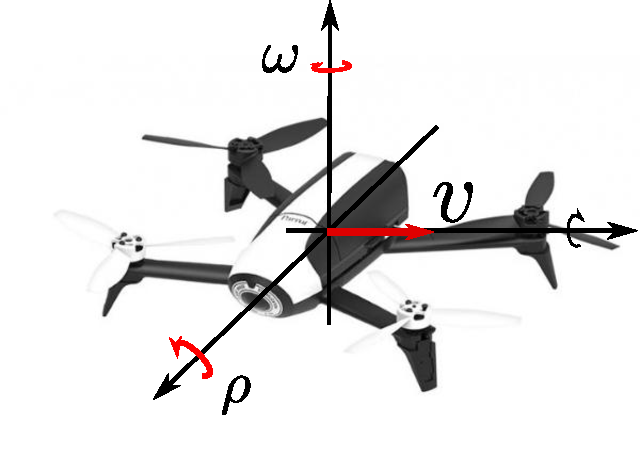
\includegraphics[width=\textwidth]{dronesteup}
\end{minipage}
\caption{Disposition des capteurs utilisés pour l'experience}
\label{fig:drone}
\end{figure}

\begin{figure}
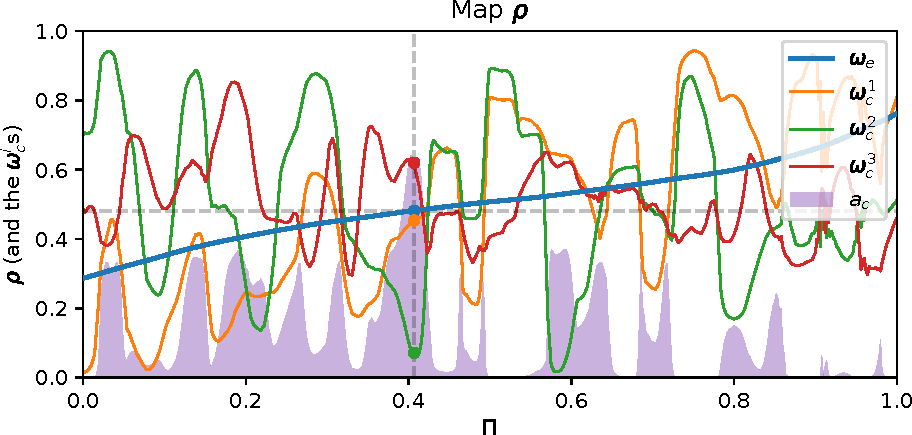
\includegraphics[width=\textwidth]{dronemap}
\caption{Disposition des poids de la carte $\rho$ après apprentissage et exemple de calcul d'activité}
\label{fig:drone_w}
\end{figure}

\subsection{Discussion}
Ici on ne cherchait pas à comparer avec des valeurs théorique, mais on observe que le drone ne tape pas les murs
Illustration de la capacité de prédiction et mémoire associative
Resistance au bruit

Calcul des dépendance entre les entrées et la commande:
PCA sur les entrées, calcul de MI après apprentissage
\section{Conclusion}





